\chapter{理论基础与相关技术}

本文主要研究DSC辅助的编码计算结果传输方法，包括面向完整重构子任务的计算结果和面向恢复子任务计算结果的线性函数。因此，本章将对涉及的理论基础和相关技术进行阐述，为后续章节所提传输机制提供理论支撑。首先，本章将介绍编码计算的基本原理，重点阐述MDS码和梯度编码方法。其次，本章将介绍经典无损DSC问题，包括完整恢复的SW定理以及恢复线性函数时使用的嵌套线性码。最后，本章将介绍编码计算下行传输利用的非正交多址技术以及凹凸过程算法等原理。



\section{编码计算}

分布式边缘计算通过将计算任务划分为多个子任务并分发至多个边缘节点并行处理来降低时延。因此，主节点需要等待所有边缘节点完成计算并返回计算结果后才能恢复原始任务的计算结果。然而， 由于边缘节点可能由于系统故障等随机因素造成计算失败，进而拖长整体的计算延迟。编码边缘计算通过引入纠删码理论向计算任务中注入冗余，可以有效缓解迟滞效应带来的影响。具体来说，在编码边缘计算场景中，主节点将原始计算任务划分为多计算子任务，并通过纠删码，生成多个编码子任务，随后将编码子任务分发给边缘节点进行计算，主节点仅需接收到部分节点的计算结果即可恢复原始任务的计算结果，从而避免等待迟滞节点。
为更清晰的展示编码边缘计算的原理，图\ref{coded edge computing}以矩阵-向量乘法为例，展示了下行传输过程，假设移动设备需要计算矩阵乘法任务$\mathbf{X}=\mathbf{A}\mathbf{b}$。利用编码边缘计算的原理，移动设备首先将计算任务按行划分为三个子矩阵$\mathbf{A}_1$、$\mathbf{A}_2$、$\mathbf{A}_3$，并利用(5,3)线性码编码成五个编码子矩阵，分别是$\mathbf{A}_1^{enc}=\mathbf{A}_1$、$\mathbf{A}_2^{enc}=\mathbf{A}_2$、$\mathbf{A}_3^{enc}=\mathbf{A}_3$、$\mathbf{A}_4^{enc}=\mathbf{A}_1+\mathbf{A}_2+\mathbf{A}_3$、$\mathbf{A}_5^{enc}=\mathbf{A}_1+2\mathbf{A}_2+3\mathbf{A}_3$。随后，移动设备将这些编码子任务分发给边缘节点并行处理，当任意三个或更多节点完成计算后，完成计算的边缘节点将它们的计算结果发送给移动设备。假设边缘节点3和边缘节点4由于随机故障成为了迟滞节点，无法完成计算任务。移动设备
在收到节点1、节点2和节点5的计算结果后即可通过$\mathbf{X}_1=\mathbf{Y}_1$、$\mathbf{X}_2=\mathbf{Y}_2$以及$\mathbf{X}_3=(\mathbf{Y}_5-\mathbf{Y}_1-2\mathbf{Y}_2)/3$恢复未编码子任务计算结果，原始计算结果$\mathbf{X}$可以通过$\mathbf{X}_1$、$\mathbf{X}_2$以及$\mathbf{X}_3$得到。

\begin{figure}[t]
	\centering
	\includegraphics[width=0.7\textwidth]{figs/SW.pdf}
	\caption{编码计算示例}
	\label{coded edge computing}
\end{figure}

\subsection{面向矩阵-向量乘法的编码计算}
考虑一个包含$N$个计算节点的分布式计算系统，以矩阵-向量乘法任务$\mathbf{X}=\mathbf{A}\mathbf{b}$为例。中心节点首先将矩阵$\mathbf{A}$按行划分为$N$个子矩阵$\left\{\mathbf{A}_i\right\}_{i=1}^N$，并将这些子矩阵分配至计算节点$[N]=\{1,2,\cdots,N\}$，执行计算子任务$\mathbf{X}_i=\mathbf{A}_i\mathbf{b}$。中心节点需要接收到所有计算节点的计算结果$\left\{\mathbf{X}_i\right\}_{i=1}^N$才能恢复原始计算任务的计算结果$\mathbf{X}$。由于分布式计算可能存在迟滞效应，即边缘节点可能由于随机故障导致计算失败，从而增加整体任务的计算时延。为了缓解迟滞效应，可以采用编码计算方法。以采用MDS码对计算任务进行编码\upcite{8002642}为例，在编码过程中，首先利用$ (N,K)$-MDS码将原始矩阵$\mathbf{A}$按行分为$ K$个子矩阵，即$ \textbf{A}=\begin{bmatrix}
	\textbf{A}_1 \\
	\textbf{A}_2 \\
	\cdots \\
	\textbf{A}_K
\end{bmatrix}$。基于MDS码构造编码矩阵$\mathbf{M}=[m_{n,i}]_{n\in[N],i\in[k]}$，利用构造的编码矩阵对划分后的$K$个子矩阵进行编码，生成$N$个编码子矩阵$\left\{\mathbf{A}_{i}^{enc}\right\}_{i=1}^N$，即
\begin{equation}
	\mathbf{A}_{n=1}^{enc}=\sum_{i=1}^K m_{n,i} \mathbf{A}_i, \quad \forall n\in[N].
\end{equation}
在完成编码后，中心节点将编码后的子矩阵$\left\{\mathbf{A}_i^{enc}\right\}_{i=1}^N$分发给$N$个边缘节点执行矩阵-向量乘法计算
\begin{equation}
	\mathbf{Y}_{n}=\mathbf{A}_n^{enc}\mathbf{b}=\sum_{i=1}^K m_{n,i} \mathbf{A}_i \mathbf{b},\quad \forall n\in[N],
\end{equation}
其中，$\mathbf{Y}_i$为编码子任务$i$的编码计算结果。
此时，中心节点最多可以容忍的迟滞者数量为$S=N-K$。当接收到计算最快的$K$个节点$\left\{\pi(1),\pi(2),\cdots,\pi(K)\right\}$的计算结果$\left\{\mathbf{Y}_{\pi(1)},\mathbf{Y}_{\pi(2)},\cdots,\mathbf{Y}_{\pi(K)}\right\}$，其中计算结果满足
\begin{equation}
	\begin{bmatrix}
	 \mathbf{Y}_{\pi(1)} \\
		 \mathbf{Y}_{\pi(2)}  \\
		\cdots   \\
		 \mathbf{Y}_{\pi(K)} 
	\end{bmatrix}=
	\begin{bmatrix}
		m_{\pi(1),1}& m_{\pi(1),2} &\cdots & m_{\pi(1),K}\\
		 m_{\pi(2),1}& m_{\pi(2),2}&\cdots & m_{\pi(1),K}\\
		\cdots & \cdots &\ddots &\cdots \\
		m_{\pi(K),1}& m_{\pi(K),2}&\cdots & m_{\pi(1),K}\	\\              
	\end{bmatrix}
	\begin{bmatrix}
		\textbf{A}_1 \\
		\textbf{A}_2 \\
		\cdots \\
		\textbf{A}_K
	\end{bmatrix}\mathbf{b}.\label{mds}
\end{equation}
根据MDS的特性，编码矩阵中任意$K$列线性无关。因此，令$\mathbf{M}$表示$[m_{\pi(i),k}]_{i,k\in[k]}$，矩阵$\mathbf{M}$为可逆矩阵。在公式（\ref{mds}）两端同时乘以$\mathbf{M}^{-1}$，则可得到原始任务的计算结果$\mathbf{X}$
\begin{equation}
		\mathbf{M}^{-1}	\begin{bmatrix}
		\mathbf{Y}_{\pi(1)} \\
		\mathbf{Y}_{\pi(2)}  \\
		\cdots   \\
		\mathbf{Y}_{\pi(K)} 
	\end{bmatrix} =	\begin{bmatrix}
	m_{\pi(1),1}& m_{\pi(1),2} &\cdots & m_{\pi(1),K}\\
	m_{\pi(2),1}& m_{\pi(2),2}&\cdots & m_{\pi(1),K}\\
	\cdots & \cdots &\ddots &\cdots \\
	m_{\pi(K),1}& m_{\pi(K),2}&\cdots & m_{\pi(1),K}\	\\              
	\end{bmatrix}^{-1}	\begin{bmatrix}
	m_{\pi(1),1}& m_{\pi(1),2} &\cdots & m_{\pi(1),K}\\
	m_{\pi(2),1}& m_{\pi(2),2}&\cdots & m_{\pi(1),K}\\
	\cdots & \cdots &\ddots &\cdots \\
	m_{\pi(K),1}& m_{\pi(K),2}&\cdots & m_{\pi(1),K}\	\\              
	\end{bmatrix}	\begin{bmatrix}
	\textbf{A}_1 \\
	\textbf{A}_2 \\
	\cdots \\
	\textbf{A}_K
	\end{bmatrix}\mathbf{b}.
\end{equation}

\subsection{面向分布式学习的编码计算}

分布式机器学习通常采用同步梯度下降算法训练大规模模型，其中大规模梯度计算在多个工作节点上并行执行。然而，如果工作节点中存在迟滞节点，将会影响整体训练速度。
梯度编码作为一种面向分布式梯度计算场景的编码计算技术，通过在计算节点间数据冗余和计算冗余，使得中心节点无需等待所有节点，仅需从部分非迟滞节点接收结果即可恢复出全局梯度，从而显著提升训练效率\upcite{halbawi2018improving,tandon2017gradient}。

考虑一个分布式学习场景，给定一个包含 $d$ 个样本的数据集 $\mathcal{D} = \{(x_i, y_i)\}_{i=1}^d$，学习的目标是寻找最优模型参数 $w^* \in \mathbb{R}^p$ 以最小化损失函数 $\mathcal{l}(\cdot)$，即
\begin{equation}
	w^* = \arg \min_{\mathbf{w}} \sum_{i=1}^d \ell(w; x_i, y_i).
\end{equation}
在梯度下降算法的第 $t$ 次迭代中，模型参数更新规则为
\begin{equation}
	w^{(t+1)} = w^{(t)} - \lambda \mathbf{g}^{(t)},\label{gc}
\end{equation}
其中 $\lambda$ 为迭代步长，$\mathbf{g}^{(t)}= \sum_{i=1}^d \nabla \ell(w^{(t)}; x_i, y_i)$ 为当前参数模型$w^{(t)}$下损失函数的梯度。

为了加快训练速度，同时降低节点存储和计算负载，分布式梯度下降方法通常被采用\upcite{halbawi2018improving}。在传统的分布式梯度下降方法中，考虑一个包含$N$个节点的系统，中心节点（参数服务器）将数据集 $\mathcal{D}$ 均匀划分为 $N$ 个互不重叠的数据分块，记为 $D_1, D_2, \dots, D_N$。每个工作节点 $i$ 仅持有数据分块 $D_i$，并计算对应的局部梯度$\mathbf{g}_i$，第$t$次的迭代的局部梯度为
\begin{equation}
	\mathbf{g}_i^{(t)} = \sum_{(x_i,y_i) \in D_i} \nabla \ell(w^{(t)}; x_i, y_i),~\forall i\in[N].
\end{equation}
 中心节点需要收集所有 $N$ 个节点的局部梯度并求和以获得全梯度，即
 \begin{equation}
 	\mathbf{g}^{(t)} = \sum_{i=1}^N \mathbf{g}_i^{(t)}=\sum_{i=1}^d\ell(w^{(t)}; x_i, y_i).
 \end{equation}
 随后，中心节点将利用得到的全梯度代入公式（\ref{gc}）中更新模型参数。

 
 然而，在传统分布式梯度下降场景中，任何一个迟滞节点的延迟都会阻塞整个系统的参数更新，从而影响训练效率。为此，梯度编码被提出缓解分布式梯度下降场景中由于迟滞节点造成的训练延迟\upcite{tandon2017gradient}。
梯度编码的核心思想是通过数据复制，让每个节点计算多个分块梯度的线性组合，从而在代数层面抵消缺失的梯度信息。首先，参数服务器将数据集$\mathcal{D}$划分为$K$个互不重叠的数据子集$\left\{D_i\right\}_{i=1}^K$，第$t$次迭代对应的局部梯度为$\left\{\mathbf{g}_i^{(t)}\right\}_{i=1}^K$。
假设系统需要容忍 $S$ 个迟滞节点（即只要有 $N-S$ 个节点完成计算，系统即可更新参数模型）。梯度编码引入了一个编码矩阵 $\mathbf{B} \in \mathbb{R}^{N \times K}$，其中第 $i$ 行向量 $\mathbf{B}_i = [B_{i1}, B_{i2}, \dots, B_{iK}]$ 决定了第 $i$ 个工作节点的计算任务，其中，若矩阵元素 $B_{ij} \neq 0$，则意味着第 $i$ 个工作节点需要存储数据分块 $D_j$ 并计算其梯度 $\mathbf{g}_j$。为容忍 $S$ 个迟滞节点，每个数据分块至少需要被复制 $S+1$ 次。
工作节点 $i$ 在本地计算其持有数据分块的梯度，并向参数服务器发送这些梯度的线性组合 $u_i$，即
	\begin{equation}
		\mathbf{u}_i = \mathbf{B}_i\mathbf{g}_j,~\forall i\in[N].
	\end{equation}

在下行传输阶段，假设参数服务器从一组非迟滞节点集合 $\mathcal{F} \subset \{1, \dots, N\}$ 中接收到了结果，且 $|\mathcal{F}| \ge N-S$。参数服务器的目标是利用接收到的编码梯度 $\{u_i\}_{i \in \mathcal{F}}$ 恢复全梯度 $\mathbf{g} = [\mathbf{g}_1~\mathbf{g}_2~\cdots~\mathbf{g}_K]^T$，其中$\mathbf{g}$表示所有局部梯度的堆叠效果，等价于寻找一组解码系数 $\mathbf{A} \in \mathbb{R}^{1 \times N}$（对于迟滞节点 $j \notin \mathcal{F}$，令 $A_j=0$），使得
\begin{equation}
	\sum_{i \in \mathcal{F}} A_i \mathbf{u}_i = \sum_{i \in \mathcal{F}} A_i \left( \sum_{j=1}^k B_{ij} \mathbf{g}_j \right) = \sum_{j=1}^k \left( \sum_{i \in \mathcal{F}} A_i B_{ij} \right) \mathbf{g}_j = \sum_{j=1}^k 1 \cdot \mathbf{g}_j
\end{equation}
该式表明，梯度编码的本质是设计一个编码矩阵 $\mathbf{B}$ 必须满足，对于任意具有 $N-S$ 个非零元素的解码向量 $\mathbf{A}$，均存在解使得 $\mathbf{A}\mathbf{B} = \mathbf{1}_{1 \times K}$（全1向量）。

 \begin{figure}[htbp]
	\centering
	\includegraphics[width=0.65\textwidth]{figs/gradient coding.pdf}
	\caption{梯度编码计算}
	\label{gradient coding}
\end{figure}

为了进一步清晰的阐述梯度编码过程，图\ref{gradient coding}展示了具体的梯度编码场景。
设系统包含 $N=3$ 个节点，数据划分为 $K=3$ 块，需容忍 $S=1$ 个迟滞节点。
节点1持有 $(D_1, D_2)$，节点2持有 $(D_2, D_3)$，节点3持有 $(D_3, D_1)$。具体的编码矩阵为$\mathbf{B}=\begin{bmatrix}
	1/2 & 1 & 0 \\
	0 & 1 & -1 \\
	1/2 & 0 & 1
\end{bmatrix}$
，即节点1发送 $u_1 = \frac{1}{2}g_1 + g_2$，节点2发送 $u_2 = g_2 - g_3$，节点3发送 $u_3 = \frac{1}{2}g_1 + g_3$。
若节点3成为迟滞节点，服务器仅收到 $u_1, u_2$。可以寻找到解码向量$\mathbf{A}=[2,-1,0]$，恢复全梯度，即服务器可以通过线性组合 $2u_1 - u_2 = 2(\frac{1}{2}g_1 + g_2) - (g_2 - g_3) = g_1 + g_2 + g_3$，即可无损恢复出全梯度。具体的编码矩阵和解码矩阵的构建可以采用循环重复编码或部分重复编码，构造方法参见文献\cite{tandon2017gradient}。


\section{分布式信源编码}
\subsection{面向独立恢复的DSC}
DSC在无线传感器网络\upcite{1208942}以及分布式视频编码\upcite{6093771}等场景中得到了广泛应用。其核心思想是多个相互不通信的信源利用信源间的相关性进行压缩，并将压缩后的信息发送到中心节点（如基站）进行联合解码。具体来说，考虑一个包含$K$个相关信源的分布式系统，假设第$k$个节点观测到的数据序列为$Y_k^n=(Y_{k,1},Y_{k,2},\cdots,Y_{k,n})$，其中$Y_{k,i}$为独立同分布(independent and identically distriubted, i.i.d)的随机变量。
下面先对香农信源编码定理进行介绍，根据香农经典信源编码定理，对于一个离散无记忆信源（Discrete Memoryless Source, DMS）$Y$，若要实现无损压缩与恢复，其编码速率 $R$ 必须不低于信源的熵 $H(Y)$ \upcite{cover1999elements}。
\begin{theorem}[香农无噪信源编码定理]\label{shannon}
	设 $Y$ 为服从概率分布 $p(y)$ 的离散无记忆信源。对于任意 $\epsilon > 0$，存在一个编码方案，当序列长度 $n$ 足够大时，能够以速率 $R$ 对该信源进行编码并以高概率无损恢复，当且仅当
	\begin{equation}
		R \geq H(Y)
	\end{equation}
	其中 $H(Y) = - \sum_{y} p(y) \log_2 p(y)$ 为信源的信息熵。
\end{theorem}
如果考虑节点间互相通信的场景下，根据逐次连续编码方法\upcite{5208477}，节点$k$可以按照编码速率$H(Y_k|Y_{k-1}\cdots Y_1)$进行压缩编码。例如，图\ref{joint decoding}展示了两个信源可以通信情况下的联合编译码场景，解码端想无损恢复$\hat{Y}_1$和$\hat{Y}_2$，则编码速率只要大于$Y_1$和$Y_2$的联合熵$H(Y_1,Y_2)$。例如，可以先对信源$Y_1$压缩到每符号传输$H(Y_1)$个比特信息。由于在编码端和解码端都已知信源$Y_1$的信息，信源$Y_2$可以直接压缩至每符号传输$H(Y_2|Y_1)$个比特信息。

然而，许多场景下，信源之间不能相互通信（如图\ref{joint decoding}所示），只能独立编码。如果采用独立信源编码方式，根据香农信源编码定理，每个节点$k$独立地对其数据进行压缩并发送给中心节点，系统所需的总下行传输速率$R_{sum}$为各节点熵的直接加和，即
\begin{equation}
	R_{sum}=\sum_{k=1}^KH(Y_k).
\end{equation}
由于编码计算（如MDS编码或梯度编码）引入了信息冗余，节点信源之间存在强相关性，即联合熵往往小于各自熵之和$H(Y_1,\cdots,Y_K)<\sum H(Y_k)$。独立编码重复传输了这些冗余信息（即互信息部分），导致了带宽资源的浪费和传输时延的增加。

\begin{figure}[htbp]
	\centering
	\includegraphics[width=0.7\textwidth]{figs/example.pdf}
	\caption{两个信源$Y_1$和$Y_2$的DSC示例}
	\label{joint decoding}
\end{figure}

为了利用分布式信源间的相关性来消除冗余信息，提升传输效率，SW定理表明，即使相关的信源之间不进行通信协作（即分布式编码），只要解码器能够联合处理这些信号，理论上也可以达到与互相通信时编码（即所有数据汇聚在一起编码）相同的压缩极限 \upcite{1055037}。下面的定理为SW定理具体定义，为DSC问题提供了理论支撑。
\begin{theorem}[Slepian-Wolf 定理]
	考虑 $K$ 个统计相关的离散无记忆信源 $Y_1, Y_2, \dots, Y_K$，其联合概率分布为 $p(y_1, \dots, y_K)$。若要以任意小的错误概率在接收端无损恢复出所有信源序列，则速率元组 $(R_1, R_2, \dots, R_K)$ 必须位于 Slepian-Wolf 区域 $\mathcal{R}_{SW}$ 内。该区域由以下不等式组定义：对于所有非空子集 $\mathcal{S} \subseteq \{1, \dots, K\}$，需满足
	\begin{equation}
		\sum_{k \in \mathcal{S}} R_k \geq H(Y_{\mathcal{S}} | Y_{\mathcal{S}^c}),
	\end{equation}
	其中 $Y_{\mathcal{S}} = \{Y_k | k \in \mathcal{S}\}$，$Y_{\mathcal{S}^c}$ 表示集合 $\mathcal{S}$ 补集对应的信源变量。特别地，总传输速率必须满足
	\begin{equation}
		\sum_{k=1}^{K} R_k \geq H(Y_1, Y_2, \dots, Y_K).
	\end{equation}
\end{theorem}

\begin{figure}[htbp]
	\centering
	\includegraphics[width=0.5\textwidth]{figs/achievable.pdf}
	\caption{两个信源$Y_1$和$Y_2$的SW可达速率区域示例}
	\label{SW}
\end{figure}
为了更清晰的展示SW定理的压缩区域，图\ref{SW}给出了两个信源$Y_1$和$Y_2$的编码速率可实现区域。SW定理表明，其总编码速率下界由联合熵决定，消除了节点间的互信息冗余。只要总速率满足联合熵约束，各节点的具体速率 $R_k$ 可以在一定范围内灵活调整。例如，节点1处于深衰落信道可以降低速率（$R_1 \approx H(Y_1 | Y_2$），而节点2信道较好可以承担更多传输任务（$R_2 \approx H(Y_2)$）。这种特性使得系统能够根据信道状态自适应地进行负载重分配，从而最小化传输瓶颈。

对于实际的SW编码，最早的相关工作尝试设计编码方案来接近图\ref{SW}中的角点A（B），等效于在解码器使用边信息$Y_2$（$Y_1$）对$Y_1$（$Y_2$）进行编码\upcite{1184140, 4697499}。其核心思想是利用虚拟信道的概念，在编码端通过随机分箱或基于伴随式的线性分组码，每个节点仅需发送其数据陪集的索引，在解码端，利用各信源间的相关性作为边信息进行联合解码。下面将简要介绍基于伴随式的DSC编码方案。具体来说，基于伴随式的DSC方案的核心在于利用一个 $(n, k)$ 线性分组码的代数结构（如LDPC码和Turbo码\upcite{910571}），通过其校验矩阵 $\mathbf{H} \in \mathbb{F}_q^{(n-k) \times n}$ 将信源空间划分为多个互不相交的陪集。
编码端在观测到信源序列 $\mathbf{Y}_2$ 后，并不直接传输原始数据，而是计算并发送其对应的伴随式 $\mathbf{s} = \mathbf{H}\mathbf{Y}_2^T$。由于伴随式的长度仅为 $n-k$，该方案将传输速率压缩至 $(n-k)/n$。在解码端，伴随式 $\mathbf{s}$ 唯一确定了 $\mathbf{Y}_2$ 所在的陪集。解码器将旁信息 $\mathbf{Y}_2$ 视为 $\mathbf{Y}_1$ 经过虚拟相关信道干扰后的观测值，并在指定的陪集内搜索与 $\mathbf{Y}_2$ 具有最大后验概率的序列 $\mathbf{\hat{Y}}_1$。这一过程将分布式信源编码问题转化为了经典的信道纠错解码问题。

\subsection{面向线性恢复的DSC}

在一些分布式计算应用中（如分布式机器学习的梯度聚合\upcite{9562559}），中心节点并不需要恢复每个节点的具体数据 $Y_k$，而只需要恢复这些数据的特定函数值 $Z = f(Y_1, \dots, Y_K)$。由于SW定理在恢复信源时恢复所有独立数据，经典SW压缩区域在恢复线性函数计算场景下的信源压缩方案往往不再是最优的。
针对线性函数计算（如梯度的加权和），Körner 和 Marton 提出了利用信源代数结构的编码理论 \upcite{1056022}。通过引入嵌套线性码（Nested linear codes），可以将传输速率与目标函数的熵推导压缩极限，而不需要传输所有源数据的联合熵。
Körner-Marton 定理最初是针对两个相关的二进制信源提出的，旨在解决模二和的线性计算问题，具体定义如下
\begin{theorem}[Körner-Marton 定理]
	设 $X$ 和 $Y$ 为两个取值于 $\{0, 1\}$ 的离散无记忆相关信源，接收端的目标是无损恢复二者的模二和 $Z = X \oplus Y$。若采用相同的线性分组码进行编码，当编码速率 $R_X$ 和 $R_Y$ 满足以下条件时，接收端可以以任意小的错误概率恢复出 $Z$：
	\begin{equation}
		R_X \geq H(Z), \quad R_Y \geq H(Z)
	\end{equation}
	其中 $H(Z) = H(X \oplus Y)$ 为目标函数的熵。
\end{theorem}

文献\cite{lim2019towards}提出了基于嵌套线性码联合典型性译码的DSC方案，将Körner-Marton 定理的结果推广到了计算任意数量的线性组合，下面的定理给出了有损情况下具体的可达速率区域。其中，文献\cite{lim2019towards}考虑一个包含$K$个节点的分布式有损计算系统（如图\ref{linearcoding}所示），具有$K+1$个相关的无记忆信源$(Y_1^n, Y_2^n,\cdots,Y_K^n,X^n)\sim \Pi_{i=1}^np_{Y_1,\cdots,Y_K}(y_1,\cdots,y_K,x)$和失真函数$d_j(\cdot),j\in[1:J]$，$J$表示要恢复的线性组合个数，$Y_k$表示节点$k$的信源，$X$是解码端的边信息。假设信源符号定义在有限域$\mathbb{F}_q$，系统需要恢复$J$个线性组合，即恢复$Y_{\mathbf{F}}=\mathbf{F}\left[Y_1,\cdots,Y_K\right]$，其中矩阵$\mathbf{F}\in \mathbb{F}_q^{J\times K}$。
\begin{figure}[htbp]
	\centering
	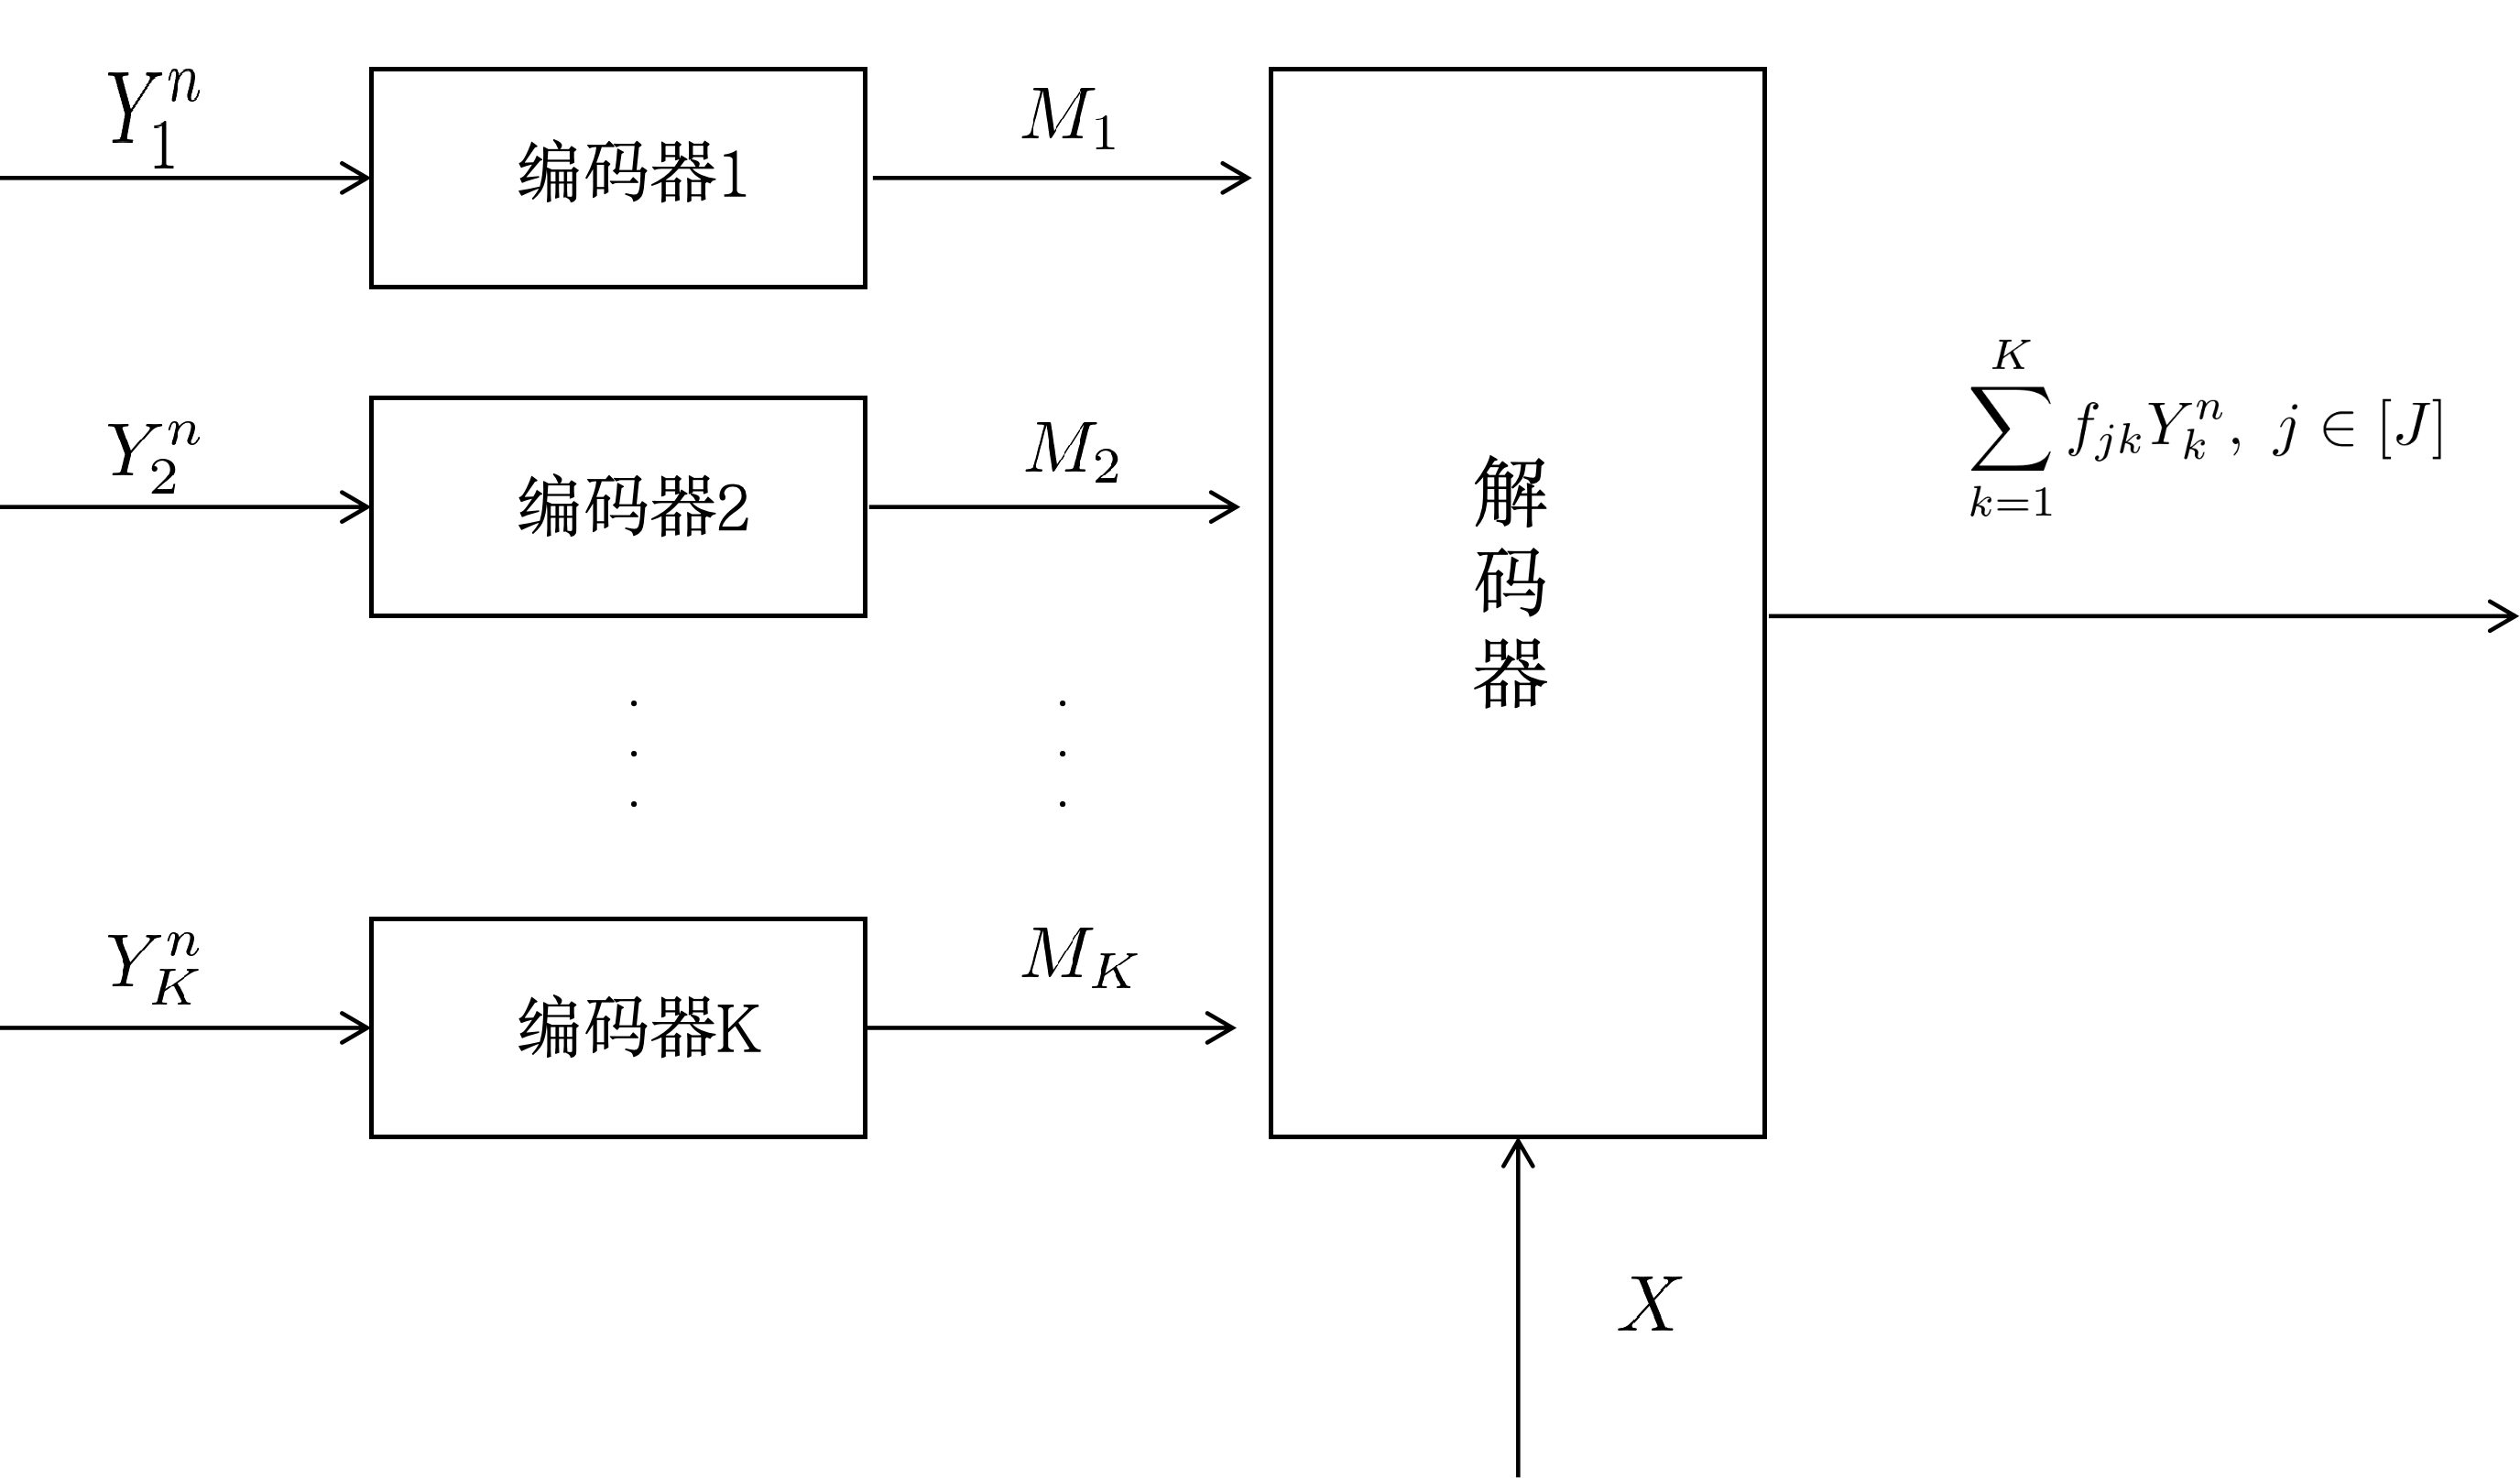
\includegraphics[width=0.65\textwidth]{linearcoding.png}
	\caption{恢复线性函数计算的DSC示例}
	\label{linearcoding}
\end{figure}

\begin{theorem}[Lim et al. \cite{lim2019towards}]\label{<theorem-chapter-2>}
	若对于某个测试信道选择$\Pi_{i=1}^rp(u_i|y_i)$，使得估计值$\hat{Y}_{\mathbf{F}}=\tilde{\mathbf{F}}[\mathbf{U}_1,\cdots,\mathbf{U}_r]^T$满足如下失真约束
	\begin{equation}
		\text{E}\left(d_j(Y_{\mathbf{F}_j}, \hat{Y}_{\mathbf{F}_j})\right)\leq d_j,~\forall j\in[1:J]
	\end{equation}
	则对于恢复系数矩阵为$\mathbf{F}\in \mathbb{R}^{J\times K}$，失真元组$(d_1,\cdots,d_J)$以及速率元组$(R_1,\cdots,R_r)$是可达的，只要它包含在以下区域$\mathcal{h}$中
	\begin{equation}
		\mathcal{h}=\bigcup_{\mathbf{E}}\bigcap_{\mathbf{C}}\bigcup_{\mathcal{S}}\bigcap_{\mathcal{T}}\left\{(R_1,\cdots,R_r)\in \mathbb{R}_+^r: \sum_{i\in\mathcal{T}}R_i>H(\hat{\mathbf{Y}}_\mathbf{E}|X,\hat{\mathbf{Y}}_{\mathbf{C}\mathbf{E}}-H(U(\mathcal{T})|Y(\mathcal{T})\right\},
	\end{equation}
	其中$\hat{\mathbf{Y}}_{\mathbf{E}}=\mathbf{E}[U_1,\cdots,U_r]^T$，$\hat{\mathbf{Y}}_{\mathbf{C}\mathbf{E}}=\mathbf{C}\mathbf{E}[U_1,\cdots,U_r]^T$，$X$为边信息，且集合运算是针对所有满足以下约束的元组（$\mathbf{E},\mathbf{C},\mathcal{S},\mathcal{T}$）进行的
	
	（a）$\mathbf{E}\in \mathbb{F}_q^{L_{\mathbf{E}\times r}}$遍历所有满秩矩阵，使得$1\leq L_{\mathbf{E}}\leq r$且span($\mathbf{E}$)$\supseteq$span($\tilde{\mathbf{F}}$)。
	
	（b）$\mathbf{C}\in \mathbb{F}_q^{L_{\mathbf{C}}\times L_{\mathbf{E}}}$遍历所有满秩矩阵（包括空矩阵），使得$0\leq L_{\mathbf{C}}< L_{\mathbf{E}}$。
	
	（c）$\mathcal{S}\subseteq[1:L_{\mathbf{E}}]$遍历所有大小为$|\mathcal{S}|=L_{\mathbf{E}}-L_{\mathbf{C}}$且满足
	\begin{equation}
		\textrm{rank}\left(\left[\begin{matrix}
			C\\
			\textbf{\textrm{I}}_{L_{\mathbf{E}}}(\mathcal{S})
		\end{matrix}\right]\right)=L_{\mathbf{E}},
	\end{equation}
	
	（d）$\mathcal{T}\subset[r]$ 遍历所有大小为$|\mathcal{T}|=L_{\mathbf{E}}-L_{\mathbf{C}}$且满足
	\begin{equation}
		\textrm{rank}\left(\left[\begin{matrix}
			\mathbf{E}(\mathcal{S})\\
			\textbf{\textrm{I}}_r([r] \backslash \mathcal{T})
		\end{matrix}\right]\right)=r.
	\end{equation}
	
\end{theorem}

\begin{proof}
	详见文献\cite{lim2019towards}第四章节证明。
\end{proof}

\begin{figure}[htbp]
	\centering
	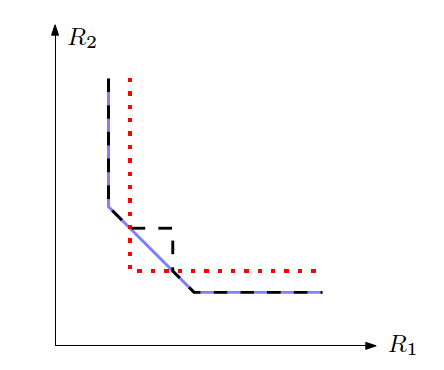
\includegraphics[width=0.45\textwidth]{nlc.png}
	\caption{两个信源基于嵌套线性码联合典型性译码的可达编码速率区域示例}
	\label{nlc}
\end{figure}
为了更清晰的阐述定理\ref{<theorem-chapter-2>}的可达速率区域，图\ref{nlc}给出了包含两个节点的系统，无损恢复一个线性组合的示例速率区域。其中，蓝色实线区域是SW可达速率区域，红色点线是Körner-Marton 可达速率区域，黑色虚线区域表示使用嵌套线性码独立恢复两个信源再进行线性计算的可达速率区域。定理\ref{<theorem-chapter-2>}可以实现Körner-Marton区域和黑色区域的并集，包含了SW区域，实现了比SW压缩更优的效果。

%\subsubsection{技术理论：嵌套线性码}
%嵌套线性码利用了有限域上线性码的群同态性质（Group Homomorphism）。一个嵌套线性码由一对线性码 $(\mathcal{C}_{\text{fine}}, \mathcal{C}_{\text{coarse}})$ 构成，满足 $\mathcal{C}_{\text{coarse}} \subset \mathcal{C}_{\text{fine}}$。其中 $\mathcal{C}_{\text{fine}}$（细码）用于保证信源的量化或覆盖，而 $\mathcal{C}_{\text{coarse}}$（粗码）用于实现分箱压缩。
%
%\begin{itemize}
%	\item \textbf{编码}：源节点 $k$ 将其观测数据序列映射到细码中的码字，并计算该码字相对于粗码的\textbf{伴随式（Syndrome）}或陪集索引。
%	\item \textbf{计算}：由于线性码的代数封闭性，接收端收到的多个伴随式的线性组合，恰好等于目标线性函数对应数据的伴随式。
%	\item \textbf{解码}：接收端直接对目标函数的伴随式进行解码，恢复出函数值。
%\end{itemize}
%
%\begin{theorem}[线性函数计算的可达速率界]
%	假设需要通过分布式网络计算 $K$ 个信源的线性组合 $Z = \sum_{k=1}^{K} c_k Y_k$，其中 $c_k$ 为有限域上的系数。若采用具有相同代数结构的嵌套线性码，当所有参与节点的编码速率 $R$ 满足以下条件时，接收端可以无损恢复目标函数 $Z$：
%	\begin{equation}
%		R \geq H(Z) = H\left(\sum_{k=1}^{K} c_k Y_k\right)
%	\end{equation}
%	更一般地，对于分布式线性函数计算问题，Körner-Marton 区域 $\mathcal{R}_{KM}$ 指出，只要速率满足以下条件即可实现函数恢复：
%	\begin{equation}
%		R_k \geq H\left(\sum_{k=1}^{K} c_k Y_k\right), \quad \forall k \in \{1, \dots, K\}
%	\end{equation}
%\end{theorem}
%
%\subsubsection{性能对比与意义}
%相较于 SW 编码，代数编码在特定场景下具有巨大的优势。例如，当两个二进制信源 $Y_1, Y_2$ 相互独立且均匀分布，但我们需要计算其模 2 和 $Z = Y_1 \oplus Y_2$ 时：
%\begin{itemize}
%	\item \textbf{SW 编码}：需恢复 $Y_1$ 和 $Y_2$，总速率 $R_{\text{sum}} \ge H(Y_1, Y_2) = 2$ bit。
%	\item \textbf{代数编码}：仅需恢复 $Z$，每个节点发送速率 $R \ge H(Z) = 1$ bit 即可（若利用广播特性可更低）。
%\end{itemize}

%在编码边缘计算中，这意味着如果任务是梯度聚合（求和），我们可以利用数据的线性结构，使得下行通信开销仅与模型参数维度相关，而与参与计算的边缘节点数量解耦，从而极大地提升大规模分布式系统的扩展性。

\section{NOMA}
% 作为5G、6G通信中的关键多址技术\cite{6G_NOMA_JEIT,NOMA6G_COMST}，
在编码计算场景中，当边缘节点完成计算任务后，需要通过下行无线信道将计算结果回传给中心节点进行恢复原始计算结果。为了提升频谱效率，下行传输考虑采用非正交多址接入技术（Non-Orthogonal Multiple Access，NOMA），采用其他多址接入技术也同样适用（如速率分割多址接入\upcite{9831440}）。
针对下一代无线通信系统对高频谱效率与海量连接的需求，非正交多址接入技术作为一种突破传统正交多址（OMA）资源分配范式的方案，受到了学术界和工业界的广泛关注\upcite{8357810}。根据资源映射方式的不同，NOMA主要分为功率域非正交多址（Power-Domain NOMA，PD-NOMA）\upcite{161197}、多用户共享接入（Multi-User Shared Access， MUSA）\upcite{170618}等。
PD-NOMA的核心思想在于通过在发射端引入叠加编码（Superposition Coding，SC），使多个用户共享同一时频资源块，并利用不同用户间信道增益的差异进行功率复用。在接收端，则采用相继干扰消除（Successive Interference Cancellation，SIC）技术，按照信号功率强度或者信道质量顺序逐层解码，从而有效缓解多用户干扰，如图\ref{noma}所示。本文后续研究均基于PD-NOMA展开（以下简称NOMA）。

\begin{figure}[htbp]
	\centering
	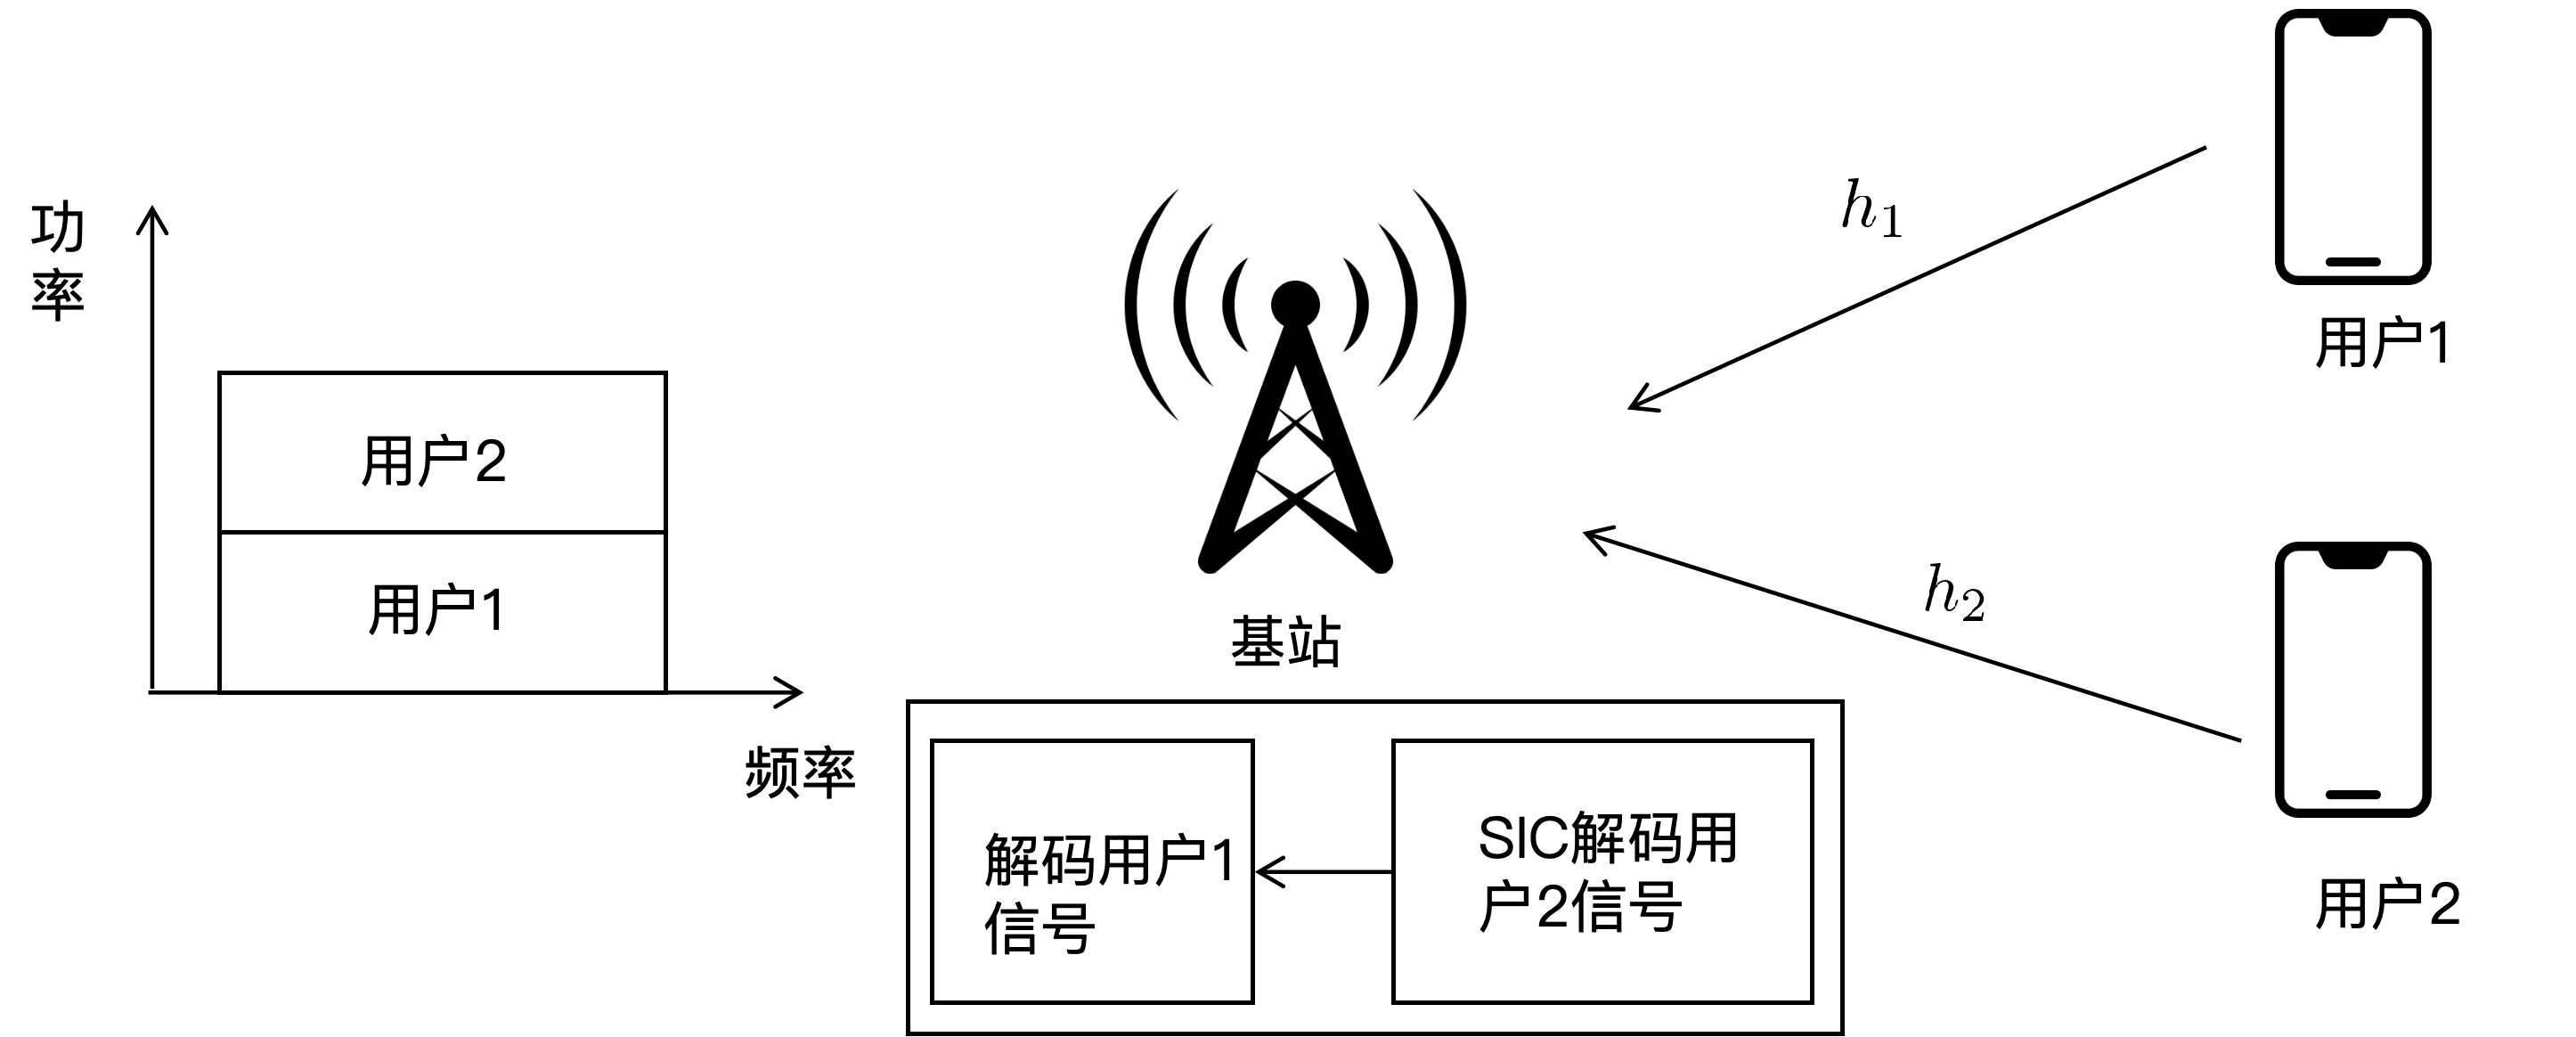
\includegraphics[width=0.75\textwidth]{NOMA.png}
	\caption{功率域NOMA示意图}
	\label{noma}
\end{figure}
考虑一个包含$N$个边缘节点的编码计算场景，当计算较快的$K$个节点完成计算后，向中心节点下行传输计算结果，记第$k$个节点发射的信号为$s_k$，其发射功率为$p_k$。中心节点接收到的叠加信号为
\begin{equation}
	y=\sum_{k=1}^K \sqrt{p_k}h_ks_k+n_w,
\end{equation}
其中，$h_n$表示第$k$个边缘节点到中心节点的信道系数，$n_w \sim \mathcal{C}\mathcal{N}(0,\sigma^2)$为加性高斯白噪声（Additive Gaussian White Noise，AWGN）。

在接收端，中心节点根据各路信号的发射功率和信道系数升序（或降序）执行SIC检测，不失一般性，假设节点间的信道增益满足
\begin{equation}
	|h_1|^2p_1\geq |h_2|^2p_2\geq \cdots \geq |h_K|^2p_K.
\end{equation}
中心节点首先解码信号$s_1$，并将其余用户信号视作干扰。在解调出$s_k$后，中心节点从总接收信号中重构并减去该分量，再进行下一级解码。在理想SIC条件下，第$k$个用户所能达到的信息传输速率为
\begin{equation}
	R_k = B\log_2\left(1+\frac{p_k|h_k|^2}{N_0B+\sum_{i=k+1}^{K}p_i|h_i|^2}\right),
\end{equation}
其中$B$为带宽，$N_0$为背景噪声功率谱密度。

\section{凹凸过程与差分凸规划理论}

在编码边缘计算的资源分配优化问题中，由于无线信道的干扰特性以及通信与计算资源的耦合关系，目标函数或约束条件往往呈现出非凸特性。直接求解此类非凸优化问题通常是 NP-hard 的。凹凸过程（Convex-Concave Procedure, CCCP）作为一种处理差分凸（Difference of Convex, DC）规划问题的算法框架，能够将复杂的非凸问题转化为一系列凸优化子问题进行迭代求解，从而高效地收敛到局部最优解。本节将详细阐述其数学模型、核心原理及求解步骤。

具体来说，差分凸规划是一类特殊的非凸优化问题，其核心思想是任何非凸的目标函数或约束函数，往往可以表示为两个凸函数之差的形式。
考虑如下标准的非凸优化问题，
\begin{equation}
	\begin{aligned}
		\min_{\mathbf{x}} \quad & f_0(\mathbf{x}) \\
		\text{s.t.} \quad & f_i(\mathbf{x}) \leq 0, \quad i = 1, \dots, m,
	\end{aligned}
\end{equation}
其中 $\mathbf{x} \in \mathbb{R}^n$ 为优化变量。若函数 $f_i(\mathbf{x})$ ($i=0,\dots,m$) 可以分解为两个凸函数 $g_i(\mathbf{x})$ 和 $h_i(\mathbf{x})$ 的差，即
\begin{equation}
	f_i(\mathbf{x}) = g_i(\mathbf{x}) - h_i(\mathbf{x}),
\end{equation}
其中 $g_i: \mathbb{R}^n \rightarrow \mathbb{R}$ 和 $h_i: \mathbb{R}^n \rightarrow \mathbb{R}$ 均为凸函数，则该问题被称为差分凸规划问题，标准形式如下
\begin{equation}
	\label{eq:dc_standard}
	\begin{aligned}
		\min_{\mathbf{x}} \quad & g_0(\mathbf{x}) - h_0(\mathbf{x}) \\
		\text{s.t.} \quad & g_i(\mathbf{x}) - h_i(\mathbf{x}) \leq 0, \quad i = 1, \dots, m.
	\end{aligned}
\end{equation}
%例如，在通信系统中，常见的香农容量公式或信干噪比（SINR）约束通常符合 DC 结构，$\log(1+\text{SINR})$ 形式的非凸函数可以拆解为：
%\begin{equation}
%	\log\left(1 + \frac{S}{I+N}\right) = \underbrace{\log(S+I+N)}_{\text{凹函数}} - \underbrace{\log(I+N)}_{\text{凹函数}}.
%\end{equation}

对于DC问题的优化，可以采用CCCP算法。CCCP 的核心原理基于凸分析中的一阶泰勒展开和最大化-最小化（Majorization-Minimization, MM）思想。其主要方法是保持 DC 结构中的凸部分 $g_i(\mathbf{x})$ 不变，而对非凸部分（即减去的凸函数 $-h_i(\mathbf{x})$）进行线性化处理。
根据凸函数的性质，对于任意可微的凸函数 $h(\mathbf{x})$，其一阶泰勒展开构成了该函数的全局下界（Global Lower Bound）。即对于任意点 $\mathbf{x}^{(k)}$，有
\begin{equation}
	h(\mathbf{x}) \geq h(\mathbf{x}^{(k)}) + \nabla h(\mathbf{x}^{(k)})^T (\mathbf{x} - \mathbf{x}^{(k)})
\end{equation}
其中 $\nabla h(\mathbf{x}^{(k)})$ 表示函数在点 $\mathbf{x}^{(k)}$ 处的梯度。
在 CCCP 的第 $k$ 次迭代中，需要寻找原问题的一个凸近似。由于 $-h_i(\mathbf{x})$ 是凹函数，利用上述不等式，可以得到 $-h_i(\mathbf{x})$ 的一个全局线性上界
\begin{equation}
	-h_i(\mathbf{x}) \leq -\left[ h_i(\mathbf{x}^{(k)}) + \nabla h_i(\mathbf{x}^{(k)})^T (\mathbf{x} - \mathbf{x}^{(k)}) \right]
\end{equation}
定义线性化后的近似函数为 $\hat{h}_i(\mathbf{x}; \mathbf{x}^{(k)})$：
\begin{equation}
	\hat{h}_i(\mathbf{x}; \mathbf{x}^{(k)}) \triangleq h_i(\mathbf{x}^{(k)}) + \nabla h_i(\mathbf{x}^{(k)})^T (\mathbf{x} - \mathbf{x}^{(k)})
\end{equation}
通过将原 DC 问题 \eqref{eq:dc_standard} 中的所有 $h_i(\mathbf{x})$ 替换为其一阶近似 $\hat{h}_i(\mathbf{x}; \mathbf{x}^{(k)})$，可以构造出第 $k$ 次迭代的凸优化子问题：
\begin{equation}
	\label{eq:cccp_subproblem}
	\begin{aligned}
		\mathbf{x}^{(k+1)} = \arg \min_{\mathbf{x}} \quad & g_0(\mathbf{x}) - \hat{h}_0(\mathbf{x}; \mathbf{x}^{(k)}) \\
		\text{s.t.} \quad & g_i(\mathbf{x}) - \hat{h}_i(\mathbf{x}; \mathbf{x}^{(k)}) \leq 0, \quad i = 1, \dots, m
	\end{aligned}
\end{equation}

由于 $g_i(\mathbf{x})$ 和 $\hat{h}_i(\mathbf{x}; \mathbf{x}^{(k)})$ 是凸函数，因此上述子问题的目标函数和约束条件均为凸函数，可以利用标准的凸优化工具（如内点法等\upcite{boyd2004convex, potra2000interior}）求解该子问题。
由于CCCP算法会阐述一个解序列$\{\mathbf{x}^{(0)},\mathbf{x}^{(1)}\cdots\}$，并且优化过程中每一步都用函数的上界来近似目标函数和约束函数，根据 MM 算法理论，该序列的目标函数值是单调非递增的，即
\begin{equation}
	f_0(\mathbf{x}^{(k+1)}) \leq f_0(\mathbf{x}^{(k)})
\end{equation}
对于原问题的目标函数有下界的情况，CCCP的算法保证了收敛性，并且CCCP 通常收敛到原非凸问题的一个驻点，即满足 Karush-Kuhn-Tucker (KKT) 条件的局部最优解 \cite{7547360}。

%\subsection{算法步骤与收敛性}
%
%基于上述原理，CCCP 求解非凸优化问题的标准步骤如下：
%
%\begin{enumerate}
%	\item \textbf{初始化}：选择一个初始可行点 $\mathbf{x}^{(0)}$，设定容忍误差 $\epsilon > 0$ 和最大迭代次数 $L_{max}$，置迭代计数器 $k=0$。
%	\item \textbf{凸化近似}：在当前点 $\mathbf{x}^{(k)}$ 处，计算所有非凸项 $h_i(\mathbf{x})$ 的梯度 $\nabla h_i(\mathbf{x}^{(k)})$。
%	\item \textbf{求解子问题}：构造并求解凸优化子问题 \eqref{eq:cccp_subproblem}，得到新的最优解 $\mathbf{x}^{(k+1)}$。
%	\item \textbf{收敛判断}：检查收敛条件 $\|\mathbf{x}^{(k+1)} - \mathbf{x}^{(k)}\| \leq \epsilon$ 或目标函数值的变化量是否小于阈值。若满足条件，则停止迭代并输出 $\mathbf{x}^* = \mathbf{x}^{(k+1)}$；否则，令 $k \leftarrow k+1$，返回步骤 2。
%\end{enumerate}




\section{本章小结}

本章系统阐述了支撑本文研究的核心理论与关键技术，为后续章节中提出的编码结构适配传输机制奠定了坚实的理论基础。
首先，介绍了编码边缘计算的基本原理，重点分析了MDS码和梯度编码（在缓解分布式计算迟滞效应中的作用。分析表明，虽然任务编码引入了计算冗余，但也使得不同边缘节点的计算结果之间产生了强相关性，这为通信环节的优化提供了物理前提。
其次，深入探讨了DSC理论。通过对比传统的独立信源编码，阐述了面向完整数据恢复的 Slepian-Wolf 定理以及面向线性函数计算的嵌套线性码（基于 Körner-Marton 定理）。这部分理论揭示了如何利用计算结果间的相关性或代数结构来逼近数据压缩的理论极限，从而降低通信开销。
再次，介绍了非正交多址接入（NOMA）技术。作为一种高效的物理层传输手段，NOMA 允许利用功率域复用实现多节点的并发传输，能够有效提升下行链路的频谱效率和连接密度。
最后，详细描述了差分凸规划（DC Programming）模型及凹凸过程（CCCP）算法。针对编码边缘计算中通信与计算资源深度耦合所导致的非凸优化难题，CCCP 提供了一套收敛性良好且高效的数学求解框架。
综上所述，编码计算产生的结构化数据、分布式信源编码提供的压缩理论、NOMA 提供的高效传输手段以及 CCCP 提供的优化方法，共同构成了本文的研究基石。在接下来的章节中，本文将基于上述理论，分别针对通用数据完整重构场景（第三章）和特定线性函数聚合场景（第四章），展开具体的传输机制设计与性能优化研究。